Die beiden Hauptkomponenten des Projekts bilden VJCMS.py und monitor.py. Neben den beiden Skripten gibt es noch eine Sammlung von Klassen, die in den Ordner utils ausgegliedert sind. Diese umfassen das Logging, Exceptions und eine Implementierung von Viola-Jones.

\begin{figure}[H]
\centering
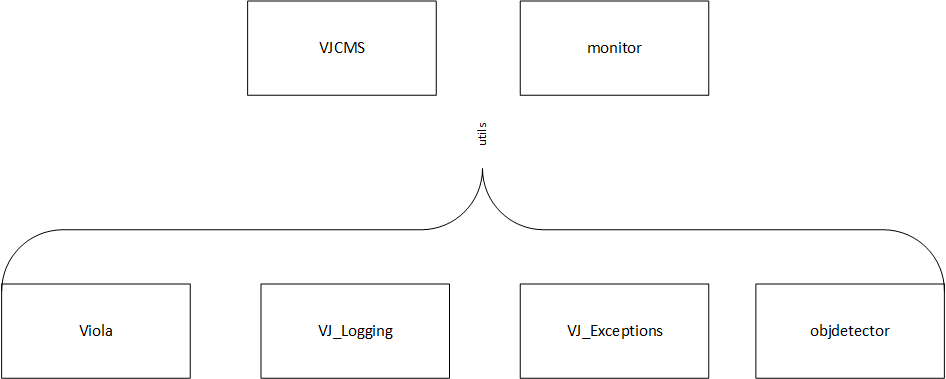
\includegraphics[width=0.7\linewidth]{img/vjcms_structure.png}
\caption{Programmaufbau}
\label{fig: structure}
\end{figure}

\subsection{VJCMS}

VJCMS bildet den Kern des Programms und übernimmt einen Großteil der Berechnungen. Neben der main-Methode befinden sich in diesem Modul Funktionen zur Ausgabe der Frames und zum Verfolgen der erkannten Objekte. Die Erkennung selbst ist wiederum in die Klasse Viola ausgelagert. 
\subsection{Viola}
\label{viola_jones}
Die Klasse Viola übernimmt die Aufbereitung der Daten des Viola-Jones Algorithmus. Der Tatsächliche Zugriff auf diese Funktionen findet in der Klasse objectdetector statt. In Viola werden die einzelnen Klassifizierer für die verschiedenen Objekte aufgerufen und die zurückgegebenen Datensätze mit den entsprechenden Labels versehen. 

\subsection{objectdetector}
Mittels dieser Klasse wird direkt auf die Funtkionalitäten von OpenCV zugregriffen und der Klassifizierer angewendet.

\subsection{VJ\_Logging}
Das Logging umfasst neben der Ausgabe auf der Konsole auch die Ausgabe in einer Datei, die im Ordner log gespeichert wird. Nachdem sowohl VJCMS als auch monitor auf diese Klasse zugreifen gibt es zwei unterschiedliche Logging-Dateien. Insgesamt gibt es 3 Arten bzw. Klassen von Meldungen, die in diesem Projekt unterschieden werden. Zum einen gibt es INFO. Hierbei handelt es sich um Meldungen die zum Beispiel angeben welche Methode gerade aufgerufen oder welcher Modus verwendet wird. Die Klasse WARNING gibt Meldungen aus, die zwar einen Fehler oder ein Problem darstellen, aber dennoch nicht zum Abbruch des Programms führen würden. Meldungen der Klasse ERROR geben Fehler oder Probleme an, die definitiv zum Abbruch oder vorzeitigen Beenden des Programmes führen. Dies muss allerdings nicht immer auf Grund einer Exception sein. In der Konsole wird kein Zeitstempel mit angegeben, sondern lediglich um welche Klasse von Meldung es sich handelt und die Meldung selbst. In dem folgenden Auszug ist eine Reihe von Logging-Ereignissen von VJCMS zu sehen. Erkannte Objekte werden ebenfalls in das Log mit eingetragen.
\begin{lstlisting}[frame=single,basicstyle=\tiny\ttfamily][H]
[Thu Feb 22 12:21:35 2018][INFO]      [main] starting program
[Thu Feb 22 12:21:35 2018][INFO]      [main] streaming to network
[Thu Feb 22 12:21:35 2018][INFO]      [main] DEBUG 1
[Thu Feb 22 12:21:35 2018][INFO]      [main] MODE 0
[Thu Feb 22 12:21:35 2018][INFO]      [main] VERBOSE 0
[Thu Feb 22 12:21:35 2018][INFO]      [detect_and_track] Begin detect_and_track
[Thu Feb 22 12:21:35 2018][INFO]      [detect_and_track] starting Thread for Viola
[Thu Feb 22 12:21:35 2018][INFO]      [detect_and_track] opening input stream
[Thu Feb 22 12:21:35 2018][OBJECT]    [Cone](351,102) (549,240)
[Thu Feb 22 12:21:35 2018][OBJECT]    [Cone](183,141) (252,180)
\end{lstlisting}

\subsection{VJ\_Exception}
Das Modul Exception enthält lediglich zwei Ausnahmeklassen. Zum einen \glqq CameraNotConnected\grqq {} und zum anderen \glqq InvalidMode\grqq .  


\subsection{monitor.py}
Monitor.py dient auschließlich der Anzeige des Streams, welcher durch VJCMS gesendet wird, falls eine Ausgabe über das Netzwerk per Parameter angegeben wurde. Dazu muss sowohl im Client als auch im Server die entsprechende IP-Adresse und Port gesetzt werden. 
